\documentclass[a4paper,class=article,border=10pt,tikz]{standalone}
\usepackage{tikz}
\usetikzlibrary{snakes,calc,positioning,patterns,angles,quotes,decorations.pathmorphing,decorations.markings,through}
\usetikzlibrary{arrows,decorations,decorations.text}
\usepackage{rotating}
\usetikzlibrary{arrows,decorations,decorations.text}
\usetikzlibrary{patterns.meta,math}




\usepackage{siunitx}

\begin{document}

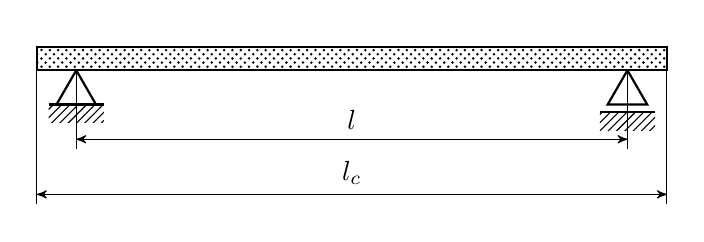
\begin{tikzpicture}

    \tikzstyle{ground}=[fill,pattern=north east lines,draw=none,minimum width=0.75cm,minimum height=0.3cm]
     \tikzstyle{close}=[draw=none,minimum width=0.75cm,minimum height=0.3cm]
    \tikzstyle{spring}=[thick,decorate,decoration={zigzag,pre length=0.3cm,post length=0.3cm,segment length=0.3cm}]
    \tikzstyle{force}=[>=stealth',ultra thick]

      \coordinate (origo) at (0,0);




    \node (part1) [draw,pattern=crosshatch dots,outer sep=0pt,thick,minimum width=8cm, minimum height=0.3cm,anchor=east,label={above:{}}] at (origo){};



\draw [thick] ([xshift=0.5cm,yshift=-0.0cm]part1.south west)--++ (-60:0.5)--++(-0.5,0) node (support_end){}--++ (60:0.5);
\node (fixed_support) [ground,outer sep=0pt,thick,anchor=north west,xshift=-0.1cm,yshift=0cm,minimum height=0.1cm ,minimum width=0.7cm]  at (support_end) {};

\draw [thick] (fixed_support.north west) -- (fixed_support.north east);
%
\draw [thick] ([xshift=-0.5cm,yshift=-0cm]part1.south east) --++ (-60:0.5) --++(-0.5,0)  node (support_start) {}  --++ (60:0.5);
%
\node (floating_support) [ground,outer sep=0pt,thick,anchor=north west,xshift=-0.1cm,yshift=-0.1cm,minimum height=0.05cm ,minimum width=0.7cm]  at (support_start) {};
%
\draw [thick] (floating_support.north west) -- (floating_support.north east);


\draw [thin] ([xshift=-0.5cm,yshift=-0cm]part1.south east) --++ (0,-1cm) node (l_dim_node_left){};
\draw [thin] ([xshift=0.5cm,yshift=-0cm]part1.south west) --++ (0,-1cm) node (l_dim_node_right){};

\draw [thin,>=stealth',<->] (l_dim_node_left.north) -- (l_dim_node_right.north) node[midway,above] {$l$};


\draw [thin] ([xshift=-0.0cm,yshift=-0cm]part1.south east) --++ (0,-1.7cm) node (lc_dim_node_left){};
\draw [thin] ([xshift=0.0cm,yshift=-0cm]part1.south west) --++ (0,-1.7cm) node (lc_dim_node_right){};

\draw [thin,>=stealth',<->] (lc_dim_node_left.north) -- (lc_dim_node_right.north) node[midway,above] {$l_c$};

\end{tikzpicture}


\end{document}
